% Original derivation-first lab briefing; the channel and numerical example are synthetic.
\documentclass[11pt,aspectratio=169]{beamer}
\usetheme{Berkeley}
\usecolortheme{dolphin}
\usepackage{amsmath,siunitx,tikz}
\usetikzlibrary{arrows.meta}
\setbeamertemplate{navigation symbols}{}
\title[Channel flow]{From a channel experiment to a scaling law}
\subtitle{A model-building laboratory briefing}
\author{Fluid mechanics laboratory}
\institute{Dimensional analysis workshop}
\date{Lab 05}
\newcommand{\Rey}{\mathrm{Re}}
\begin{document}
\begin{frame}[plain]\titlepage\end{frame}
\section{Observe}
\begin{frame}{Start by drawing the experiment}
\begin{figure}
\centering
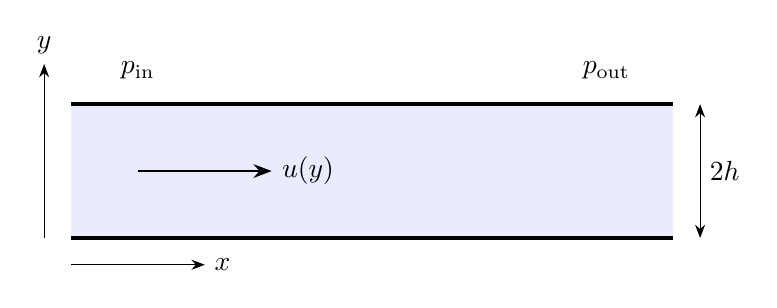
\begin{tikzpicture}[>=Stealth,scale=.85]
\fill[blue!8] (0,0) rectangle (9,2);
\draw[very thick] (0,0)--(9,0) (0,2)--(9,2);
\draw[<->] (9.4,0)--node[right]{$2h$}(9.4,2);
\draw[->,thick] (1,1)--(3,1) node[right]{$u(y)$};
\draw[->] (-.4,0)--(-.4,2.6) node[above]{$y$};
\draw[->] (0,-.4)--(2,-.4) node[right]{$x$};
\node at (1,2.5) {$p_{\mathrm{in}}$};\node at (8,2.5) {$p_{\mathrm{out}}$};
\end{tikzpicture}
\caption{Wide planar channel; stationary walls at $y=\pm h$. Sketch not to scale.}
\end{figure}
Measure geometry, pressure drop and flow rate before deciding which equation to simplify.
\end{frame}
\begin{frame}{Name the assumptions that remove terms}
\begin{itemize}[<+->]
\item Newtonian incompressible fluid with constant $\rho$ and $\mu$.
\item Steady, fully developed flow far from the entrance.
\item Width much larger than the wall separation.
\item Velocity $\mathbf{u}=(u(y),0,0)$ and constant pressure gradient.
\end{itemize}
\begin{alertblock}{Scope}
This model does not describe the entrance region or a turbulent channel.
\end{alertblock}
\end{frame}
\section{Derive}
\begin{frame}{Reduce the momentum equation, one assumption at a time}
\begin{align*}
 \rho\left(\frac{\partial\mathbf{u}}{\partial t}+\mathbf{u}\cdot\nabla\mathbf{u}\right)
 &=-\nabla p+\mu\nabla^2\mathbf{u},\\
 0&=-\frac{dp}{dx}+\mu\frac{d^2u}{dy^2}.
\end{align*}
For the stated unidirectional fully developed ansatz, the convective term vanishes even before a small-Reynolds-number approximation.
\end{frame}
\begin{frame}{Boundary conditions determine the integration constants}
\[
 u(\pm h)=0,\qquad G=-\frac{dp}{dx}>0.
\]
\begin{align*}
 u''(y)&=-G/\mu,\\
 u(y)&=\frac{G}{2\mu}(h^2-y^2),\\
 q&=\int_{-h}^{h}u(y)\,dy=\frac{2Gh^3}{3\mu}.
\end{align*}
Here $q$ is volume flow per unit width, not total volume flow.
\end{frame}
\begin{frame}{Check units before inserting values}
\begin{columns}[T]
\begin{column}{.52\textwidth}
\begin{block}{Dimensions}
$[G]=\mathrm{Pa\,m^{-1}}$, $[\mu]=\mathrm{Pa\,s}$.
\[
 [Gh^3/\mu]=\mathrm{m^2\,s^{-1}}.
\]
\end{block}
\end{column}
\begin{column}{.43\textwidth}
\begin{exampleblock}{Illustrative inputs}
$h=\SI{1}{\milli\metre}$, $G=\SI{100}{\pascal\per\metre}$,
$\mu=\SI{1}{\milli\pascal\second}$ give
$q\approx\SI{6.67e-5}{\metre\squared\per\second}$.
\end{exampleblock}
\end{column}
\end{columns}
\end{frame}
\section{Test}
\begin{frame}{A dimensionless profile collapses the family}
Let $\eta=y/h$ and $u_{\max}=Gh^2/(2\mu)$.
\[
 \frac{u}{u_{\max}}=1-\eta^2,\qquad -1\leq\eta\leq1.
\]
\begin{enumerate}
\item Normalize each measured profile by its own peak speed.
\item Compare shape before comparing amplitude.
\item Inspect near-wall residuals for systematic errors.
\end{enumerate}
\end{frame}
\begin{frame}{Use disagreement to choose the next measurement}
\begin{description}
\item[Asymmetry] Check alignment and wall placement.
\item[Wrong amplitude] Recheck pressure calibration, viscosity and the gap.
\item[Wrong shape] Revisit entrance effects and the fully developed assumption.
\end{description}
\pause
\alert{Sensitivity:} because $q\propto h^3$, a small relative gap error enters with a factor of about three.
\end{frame}
\begin{frame}{The laboratory handoff}
\begin{block}{Submit}
One dimensional check, one normalized profile, an uncertainty estimate, and one proposed falsification of the model.
\end{block}
\small
Background: \href{https://davidtong.org/teaching/fluid-mechanics/}{David Tong, Fluid Mechanics, Cambridge lecture notes}.
\medskip
All geometry and numerical inputs in this laboratory example are original teaching constructions.
\end{frame}
\end{document}
